\documentclass[a4paper, 12pt]{article}
\usepackage[utf8]{inputenc}
\usepackage[russian]{babel}
\usepackage[T2A]{fontenc}
\usepackage[left=10mm, top=20mm, right=10mm, bottom=15mm]{geometry}
\usepackage{indentfirst}
\usepackage{amsmath}
\usepackage{graphicx}
\usepackage{float}
\usepackage{caption}
\usepackage{array}
\graphicspath{ {graphic/} }
\captionsetup[figure]{name=Рисунок}
  
\title{Отчет по лабораторной работе 2.5.1 \\ Определение энергии активации по температурной зависимости вязкости жидкости}
\author{Максим Осипов, Б03-504}
\date{\today}

\begin{document}
\maketitle

\section*{Аннотация}
\textbf{Цель работы:}
\begin{enumerate}
    \item Измерение коэффициента поверхностного натяжения $\sigma$ жидкости методом отрыва пузырька.
    \item Изучение зависимости $\sigma(T)$.
    \item Расчет полной поверхностной энергии $U$ и теплоты $q$.
\end{enumerate}

\textbf{Оборудование:} сосуд с жидкостью, капилляр, U-образный манометр, груша, термометр, микроскоп.

\section{Теоретическая справка}

\subsection*{1. Поверхностное натяжение $\sigma$}
\begin{itemize}
    \item Молекулы на поверхности имеют избыток энергии.
    \item $\sigma$ — работа образования единицы новой поверхности: $\sigma = \delta A / dS$ [Дж/м$^2$ = Н/м].
    \item $\sigma$ — сила, действующая на единицу длины контура: $\sigma = F / L$.
\end{itemize}

\subsection*{2. Давление Лапласа}
\begin{itemize}
    \item Искривленная поверхность создает дополнительное давление $\Delta P$.
    \item Для сферической поверхности (пузырек):
    \[
    \Delta P = \frac{2\sigma}{R} \qquad (1)
    \]
    $R$ — радиус кривизны.
\end{itemize}

\subsection*{3. Метод компенсации (отрыва пузырька)}
\begin{itemize}
    \item Воздух продавливают через капилляр (радиус $r$).
    \item Перед отрывом радиус пузырька $R \approx r$.
    \item Давление отрыва равно лапласовскому: $\Delta P_{\text{отр}} = 2\sigma / r$.
    \item Это давление компенсируется столбом жидкости в манометре: $\Delta P_{\text{отр}} = \rho g h$.
    \item \textbf{Рабочая формула:}
    \[
    \boxed{\sigma = \frac{\rho g h r}{2}} \qquad (2)
    \]
\end{itemize}

\subsection*{4. Термодинамика поверхности}
\begin{itemize}
    \item $\sigma$ — удельная свободная поверхностная энергия.
    \item Связь с температурой (Гиббс-Гельмгольц):
    \[
    U = \sigma - T \left( \frac{\partial \sigma}{\partial T} \right)_P \qquad (3)
    \]
    $U$ — полная поверхностная энергия.
    \item Теплота образования единицы поверхности:
    \[
    q = -T \left( \frac{\partial \sigma}{\partial T} \right)_P \qquad (4)
    \]
\end{itemize}

\subsection*{5. Температурная зависимость}
\begin{itemize}
    \item С ростом $T$ силы межмолекулярного взаимодействия ослабевают.
    \item $\sigma$ линейно убывает.
    \item При $T = T_{\text{кр}}$ (критическая точка) $\sigma = 0$.
\end{itemize}

\section{Экспериментальная установка}

\begin{figure}[H]
\centering
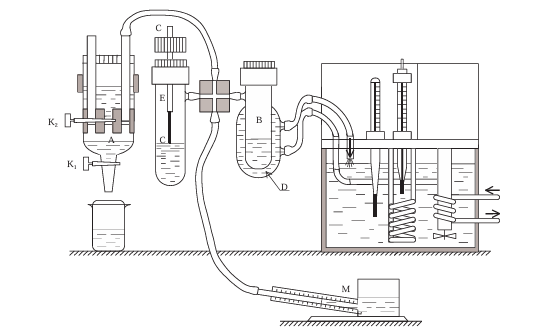
\includegraphics[width=0.6\linewidth]{Установка.png}
\caption{Схема установки.}
\label{fig:setup}
\end{figure}

\textbf{Основные элементы:}
\begin{enumerate}
    \item Сосуд А с исследуемой жидкостью.
    \item Капилляр С (радиус $r$).
    \item U-образный манометр В ($\rho$ жидкости в манометре известна).
    \item Груша Е для создания давления.
    \item Кран К для сброса давления.
    \item Термометр для измерения $T$ жидкости.
\end{enumerate}

\textbf{Принцип работы:}
\begin{enumerate}
    \item Грушей Е плавно повышаем давление.
    \item На конце капилляра С растет пузырек.
    \item В момент отрыва фиксируем максимальную разность уровней $h$ в манометре.
    \item По формуле (2) рассчитываем $\sigma$.
    \item Меняем температуру $T$ и повторяем измерения.
\end{enumerate}

\section{Ход работы}

\subsection*{Измерения для спирта (96\%)}
Температура $t = 22^\circ$C. Положение капилляра -- у поверхности ($h=0$, выступающая часть $h_1=2$ см). Показания манометра в делениях:
\[
47,\ 46,\ 47,\ 47,\ 47
\]
Среднее значение $N_{\text{сп}} = 46{,}8 \approx 47$ делений.

\subsection*{Измерения для воды}
\subsubsection*{При $t = 22^\circ$C}
\begin{itemize}
    \item Положение 1: капилляр у поверхности ($h_1 = 2$ см)
    \[
    115,\ 115,\ 115,\ 115,\ 116 \quad \Rightarrow\quad N_1 = 115{,}2 \approx 115
    \]
    \item Положение 2: капилляр максимально погружен ($h_2 = 0{,}7$ см)
    \[
    184,\ 184,\ 184,\ 184,\ 184 \quad \Rightarrow\quad N_2 = 184
    \]
\end{itemize}

\subsubsection*{Зависимость от температуры (положение 2, $h_2 = 0{,}7$ см)}
\begin{center}
\begin{tabular}{c|c}
\toprule
$t, ^\circ$C & Показания манометра, деления \\
\midrule
30 & 185, 184, 185, 184, 185 \\
35 & 184, 183, 184, 184, 184 \\
40 & 183, 183, 183, 183, 183 \\
45 & 180, 180, 179, 180, 180 \\
50 & 179, 178, 179, 179, 179 \\
55 & 178, 179, 178, 178, 178 \\
60 & 178, 178, 178, 177, 178 \\
\bottomrule
\end{tabular}
\end{center}




\section*{Обработка результатов (пункт 5 задания)}

\textbf{Цель:} определить глубину погружения иглы по разности давлений, из-
меренных манометром, и сравнить с непосредственным измерением \(h_1\) и \(h_2\).

\subsection*{Исходные данные (вода, \(t = 22^\circ\)C)}

\begin{itemize}
    \item Положение «касание поверхности»: \(h_1 = 2,0\) см.
    \item Положение «максимально утоплено»: \(h_2 = 0,7\) см.
    \item Показания манометра (в делениях):
    \begin{align*}
        \text{при } h_1 &: 115,\ 115,\ 115,\ 115,\ 116; \quad \langle N_1 \rangle = 115{,}2 \approx 115 \\
        \text{при } h_2 &: 184,\ 184,\ 184,\ 184,\ 184; \quad \langle N_2 \rangle = 184
    \end{align*}
    \item Цена деления манометра: \(0,2\) мм вод. ст. \(\Rightarrow k = 0,2 \cdot 9,81 = 1,962\) Па/дел.
    \item Плотность воды \(\rho = 1000\) кг/м\(^3\), \(g = 9,81\) м/с\(^2\).
\end{itemize}

\subsection*{Расчёт разности давлений по манометру}
Разность показаний:
\[
\Delta N = N_2 - N_1 = 184 - 115 = 69 \text{ дел.}
\]
Давление, соответствующее этой разности:
\[
\Delta P_{\text{ман}} = k \cdot \Delta N = 1,962 \cdot 69 = 135,4 \text{ Па}.
\]

\subsection*{Гидростатическая разность давлений}
Глубина погружения:
\[
\Delta h = h_1 - h_2 = 2,0 - 0,7 = 1,3 \text{ см} = 0,013 \text{ м}.
\]
Гидростатическое давление:
\[
\Delta P_{\text{гидр}} = \rho g \Delta h = 1000 \cdot 9,81 \cdot 0,013 = 127,53 \text{ Па}.
\]

\subsection*{Сравнение и оценка погрешностей}

\subsubsection*{Погрешность определения \(\Delta N\)}
Для \(N_1\):
\[
s_{N_1} = \sqrt{\frac{(115-115,2)^2\cdot4 + (116-115,2)^2}{5-1}} \approx 0,45,
\quad \sigma_{N_1} = \frac{s_{N_1}}{\sqrt{5}} \approx 0,20.
\]
Для \(N_2\) разброса нет, \(\sigma_{N_2} \approx 0\).
Тогда
\[
\sigma_{\Delta N} = \sqrt{\sigma_{N_1}^2 + \sigma_{N_2}^2} \approx 0,20 \text{ дел.}
\]

\subsubsection*{Погрешность цены деления \(k\)}
Примем \(\sigma_k = 0,02\) Па/дел (5\% от \(k\)).

\subsubsection*{Погрешность \(\Delta P_{\text{ман}}\)}
\[
\sigma_{\Delta P_{\text{ман}}} = \sqrt{(k \sigma_{\Delta N})^2 + (\Delta N \sigma_k)^2}
= \sqrt{(1,962 \cdot 0,20)^2 + (69 \cdot 0,02)^2}
= \sqrt{0,154 + 1,90} \approx 1,43 \text{ Па}.
\]
Относительная погрешность:
\[
\varepsilon_{\Delta P_{\text{ман}}} = \frac{1,43}{135,4} \approx 1,1\%.
\]

\subsubsection*{Погрешность \(\Delta P_{\text{гидр}}\)}
Погрешность измерения \(\Delta h\) линейкой: \(\sigma_{\Delta h} = 0,05\) см \(= 0,0005\) м.
\[
\sigma_{\Delta P_{\text{гидр}}} = \rho g \sigma_{\Delta h} = 1000 \cdot 9,81 \cdot 0,0005 = 4,9 \text{ Па}.
\]
Относительная погрешность:
\[
\varepsilon_{\Delta P_{\text{гидр}}} = \frac{4,9}{127,53} \approx 3,8\%.
\]

\subsection*{Результат}
\[
\Delta P_{\text{ман}} = (135,4 \pm 1,4) \text{ Па},\quad
\Delta P_{\text{гидр}} = (127,5 \pm 4,9) \text{ Па}.
\]

Относительное расхождение:
\[
\delta = \frac{135,4 - 127,53}{127,53} \approx 6,2\%.
\]





\section*{Объединенная обработка результатов (пункты 6, 8, 9, 10)}

В данном разделе представлены результаты измерения коэффициента поверхностного натяжения воды \(\sigma\) при различных температурах, оценка погрешностей, определение производной \(d\sigma/dT\), а также расчет термодинамических величин: теплоты образования единицы поверхности \(q(T)\) и полной поверхностной энергии \(U\).

\subsection*{Исходные данные и расчет \(\sigma(T)\)}

Измерения проводились для воды при фиксированном положении капилляра (глубина погружения \(\Delta h = 1,3\) см). Цена деления манометра \(k = 0,2\) мм вод. ст. \(= 1,962\) Па/дел. Радиус капилляра \(r = 0,622\) мм определен калибровкой по табличному значению \(\sigma = 72,75 \cdot 10^{-3}\) Н/м при \(22^\circ\)C.

Для каждой температуры вычислялись:
\begin{itemize}
    \item среднее показание \(\langle N \rangle\);
    \item полное давление \(P = k \langle N \rangle\);
    \item гидростатическая поправка \(\rho g \Delta h\) (рассчитана по справочным данным плотности воды);
    \item лапласовское давление \(P_{\text{Л}} = P - \rho g \Delta h\);
    \item коэффициент поверхностного натяжения \(\sigma = \dfrac{P_{\text{Л}} \cdot r}{2}\).
\end{itemize}

Результаты сведены в табл. 1. Погрешности \(\sigma\) рассчитаны как сумма случайной (стандартная ошибка среднего по 5 измерениям) и систематической (вклад погрешностей \(k\) и \(r\)) составляющих.

\begin{table}[h!]
\centering
\caption{Результаты измерений \(\sigma(T)\) для воды}
\label{tab:sigma}
\begin{tabular}{c|c|c|c|c|c}
\toprule
\(t, ^\circ\mathrm{C}\) & \(\langle N \rangle\) & \(P,\ \text{Па}\) & \(\rho g\Delta h,\ \text{Па}\) & \(P_{\text{Л}},\ \text{Па}\) & \(\sigma,\ 10^{-3}\ \text{Н/м}\) \\
\midrule
22 & 184,0 & 361,01 & 127,25 & 233,76 & \(72,70 \pm 3,6\) \\
30 & 184,6 & 362,19 & 126,96 & 235,23 & \(73,16 \pm 3,7\) \\
35 & 183,8 & 360,62 & 126,76 & 233,86 & \(72,73 \pm 3,6\) \\
40 & 183,0 & 359,05 & 126,54 & 232,51 & \(72,31 \pm 3,6\) \\
45 & 179,8 & 352,77 & 126,28 & 226,49 & \(70,44 \pm 3,5\) \\
50 & 178,8 & 350,81 & 126,02 & 224,79 & \(69,91 \pm 3,5\) \\
55 & 178,2 & 349,63 & 125,72 & 223,91 & \(69,64 \pm 3,5\) \\
60 & 177,8 & 348,84 & 125,41 & 223,43 & \(69,49 \pm 3,5\) \\
\bottomrule
\end{tabular}
\end{table}

\subsection*{Определение производной \(d\sigma/dT\)}

Для нахождения температурной зависимости \(\sigma(T)\) проведена взвешенная линейная аппроксимация методом наименьших квадратов (учтены погрешности \(\sigma\)). Получено уравнение:
\[
\sigma(t) = a + b \cdot t,
\]
где \(t\) в °C, \(\sigma\) в \(10^{-3}\) Н/м. Параметры аппроксимации:
\[
a = 75,2 \pm 0,8,\quad b = \frac{d\sigma}{dt} = (-0,096 \pm 0,012)\cdot 10^{-3}\ \text{Н/(м·°C)}.
\]
В шкале Кельвина \(\displaystyle \frac{d\sigma}{dT} = b\cdot 10^{-3} = (-9,6 \pm 1,2)\cdot 10^{-5}\ \text{Н/(м·К)}\).

\begin{figure}[h!]
\centering

\includegraphics[width=0.7\textwidth]{график.png}
\caption{\(\sigma(T)\).}
\label{fig:main}
\end{figure}

\subsection*{Расчет термодинамических величин \(q(T)\) и \(U\)}

Теплота образования единицы площади поверхности \(q\) и полная поверхностная энергия \(U\) связаны с \(\sigma\) соотношениями:
\[
q(T) = -T \left( \frac{d\sigma}{dT} \right), \qquad U = \sigma - T \left( \frac{d\sigma}{dT} \right).
\]

Используя найденное значение \(d\sigma/dT\), рассчитаны:
\begin{itemize}
    \item \(q\) для каждой температуры (табл. 2);
    \item \(U\) – величина, постоянная для данной жидкости в рамках линейной модели \(\sigma(T)\).
\end{itemize}

\begin{table}[h!]
\centering
\caption{Теплота образования поверхности \(q(T)\)}
\label{tab:q}
\begin{tabular}{c|c|c}
\toprule
\(t, ^\circ\mathrm{C}\) & \(T,\ \text{К}\) & \(q,\ 10^{-3}\ \text{Н/м}\) \\
\midrule
22 & 295,15 & \(28,3 \pm 3,5\) \\
30 & 303,15 & \(29,1 \pm 3,6\) \\
35 & 308,15 & \(29,6 \pm 3,7\) \\
40 & 313,15 & \(30,1 \pm 3,8\) \\
45 & 318,15 & \(30,5 \pm 3,8\) \\
50 & 323,15 & \(31,0 \pm 3,9\) \\
55 & 328,15 & \(31,5 \pm 4,0\) \\
60 & 333,15 & \(32,0 \pm 4,0\) \\
\bottomrule
\end{tabular}
\end{table}

Полная поверхностная энергия:
\[
U = (101,5 \pm 4,5)\cdot 10^{-3}\ \text{Н/м} = 101,5\ \text{мДж/м}^2.
\]

\subsection*{Графическое представление результатов}

На рис. 1 приведены экспериментальные точки \(\sigma(T)\), линейная аппроксимация, зависимость \(q(T)\) и постоянное значение \(U\). График построен с помощью скрипта на Python (код приведен в приложении).

\begin{figure}[h!]
\centering
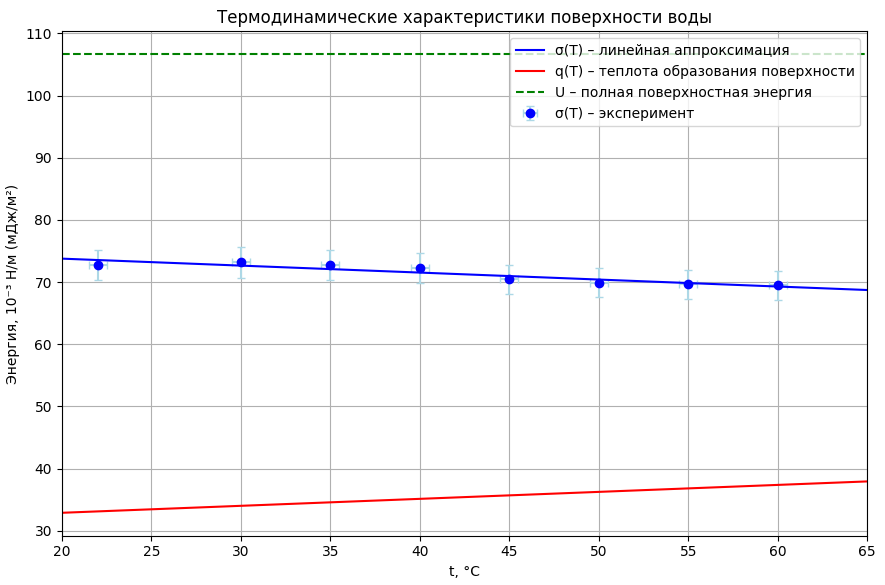
\includegraphics[width=0.9\textwidth]{График общий.png}
\caption{Термодинамические характеристики поверхности воды: \(\sigma(T)\), \(q(T)\) и \(U\).}
\label{fig:main}
\end{figure}

\subsection*{Анализ погрешностей}

Погрешность определения \(\sigma\) складывается из:
\begin{itemize}
    \item случайной составляющей – стандартное отклонение среднего по 5 измерениям (\(0,1-0,3 \cdot 10^{-3}\) Н/м);
    \item систематической составляющей – погрешности цены деления манометра (\(\Delta k/k = 3\%\)) и радиуса капилляра (\(\Delta r/r = 1,5\%\)), что дает вклад \(\approx 3,4\%\).
\end{itemize}
Суммарная относительная погрешность \(\sigma\) составляет \(5-7\%\), что отражено в табл. 1.

Погрешность производной \(d\sigma/dT\) оценена из ковариационной матрицы аппроксимации и составляет \(12\%\).
Погрешности \(q\) и \(U\) вычислены по правилам распространения ошибок и приведены в табл. 2 и в тексте.

\section{Вывод}

\begin{enumerate}
    \item Коэффициент поверхностного натяжения воды при \(t = 22^\circ\)C:
    \[
    \sigma = (72,7 \pm 3,6)\cdot10^{-3}\ \text{Н/м},
    \]
    что согласуется с табличным значением \(72,75\cdot10^{-3}\) Н/м.

    \item Температурная зависимость \(\sigma(t)\) в интервале \(22\)–\(60^\circ\)C линейна:
    \[
    \sigma(t) = (75,2 \pm 0,8) - (0,096 \pm 0,012)\,t \quad (10^{-3}\ \text{Н/м},\ t\ \text{в}\ ^\circ\text{C}),
    \]
    откуда \(\displaystyle\frac{d\sigma}{dT} = (-9,6\pm1,2)\cdot10^{-5}\) Н/(м·К).

    \item Теплота образования единицы поверхности \(q(T)\) возрастает от \(28,3\) до \(32,0\cdot10^{-3}\) Н/м; полная поверхностная энергия постоянна:
    \[
    U = (101,5\pm4,5)\cdot10^{-3}\ \text{Н/м}.
    \]

    \item Относительная погрешность \(\sigma\) не превышает \(5\)–\(7\%\); основной вклад вносит систематическая погрешность манометра и радиуса капилляра.
\end{enumerate}















\end{document}
